%!TEX root = ../main.tex
\section{Polynomial Systems, Polynomial Feedback}
\label{sec:poly}

\begin{figure*}
    \centering
    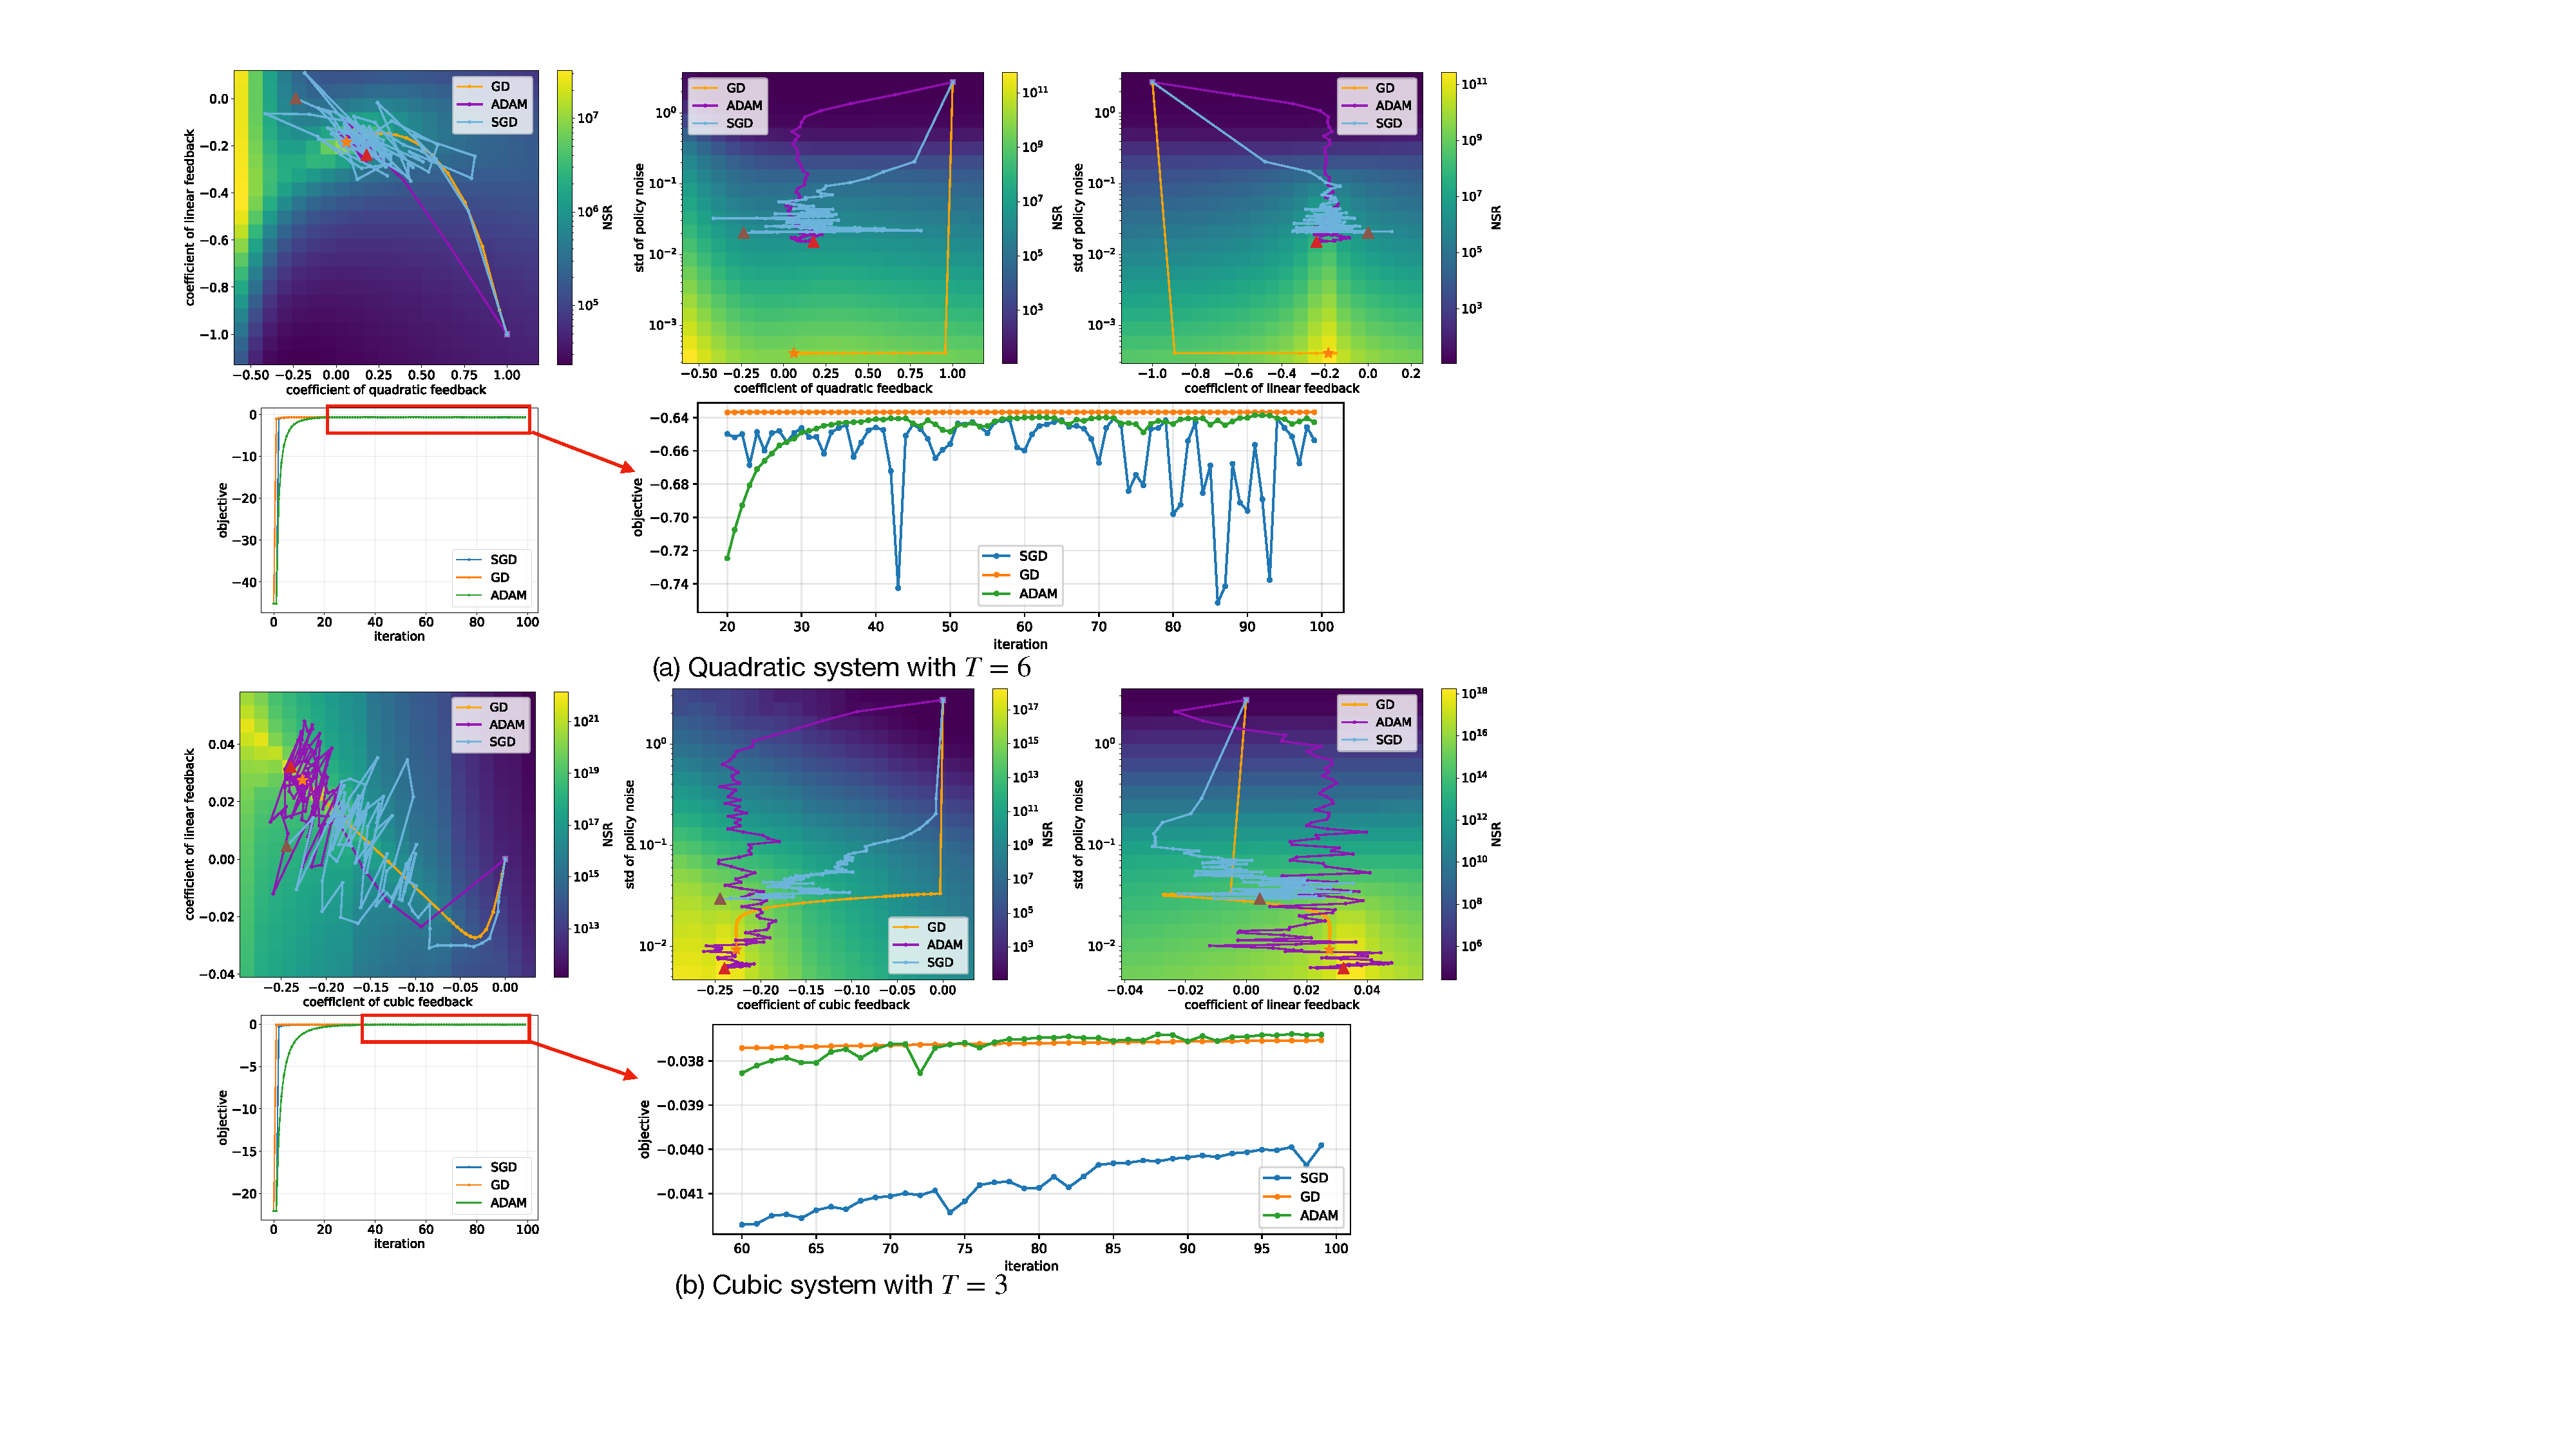
\includegraphics[width=0.9\textwidth]{figure/ratio_map_poly.pdf}
    \caption{NSR and objective along optimization trajectories on polynomial systems. (a): quadratic system; (b): cubic system. {Top}: optimizer trajectories and NSR landscape; {Bottom}: learning curves. The NSR increases when approaching the optimal policy, as in linear systems. GD consistently approaches the optimum while SGD and Adam may get stuck in high-NSR regions.}
    \label{fig:poly-variance-traj}
    \vspace{-3mm}
\end{figure*}

\begin{figure*}
    \centering
    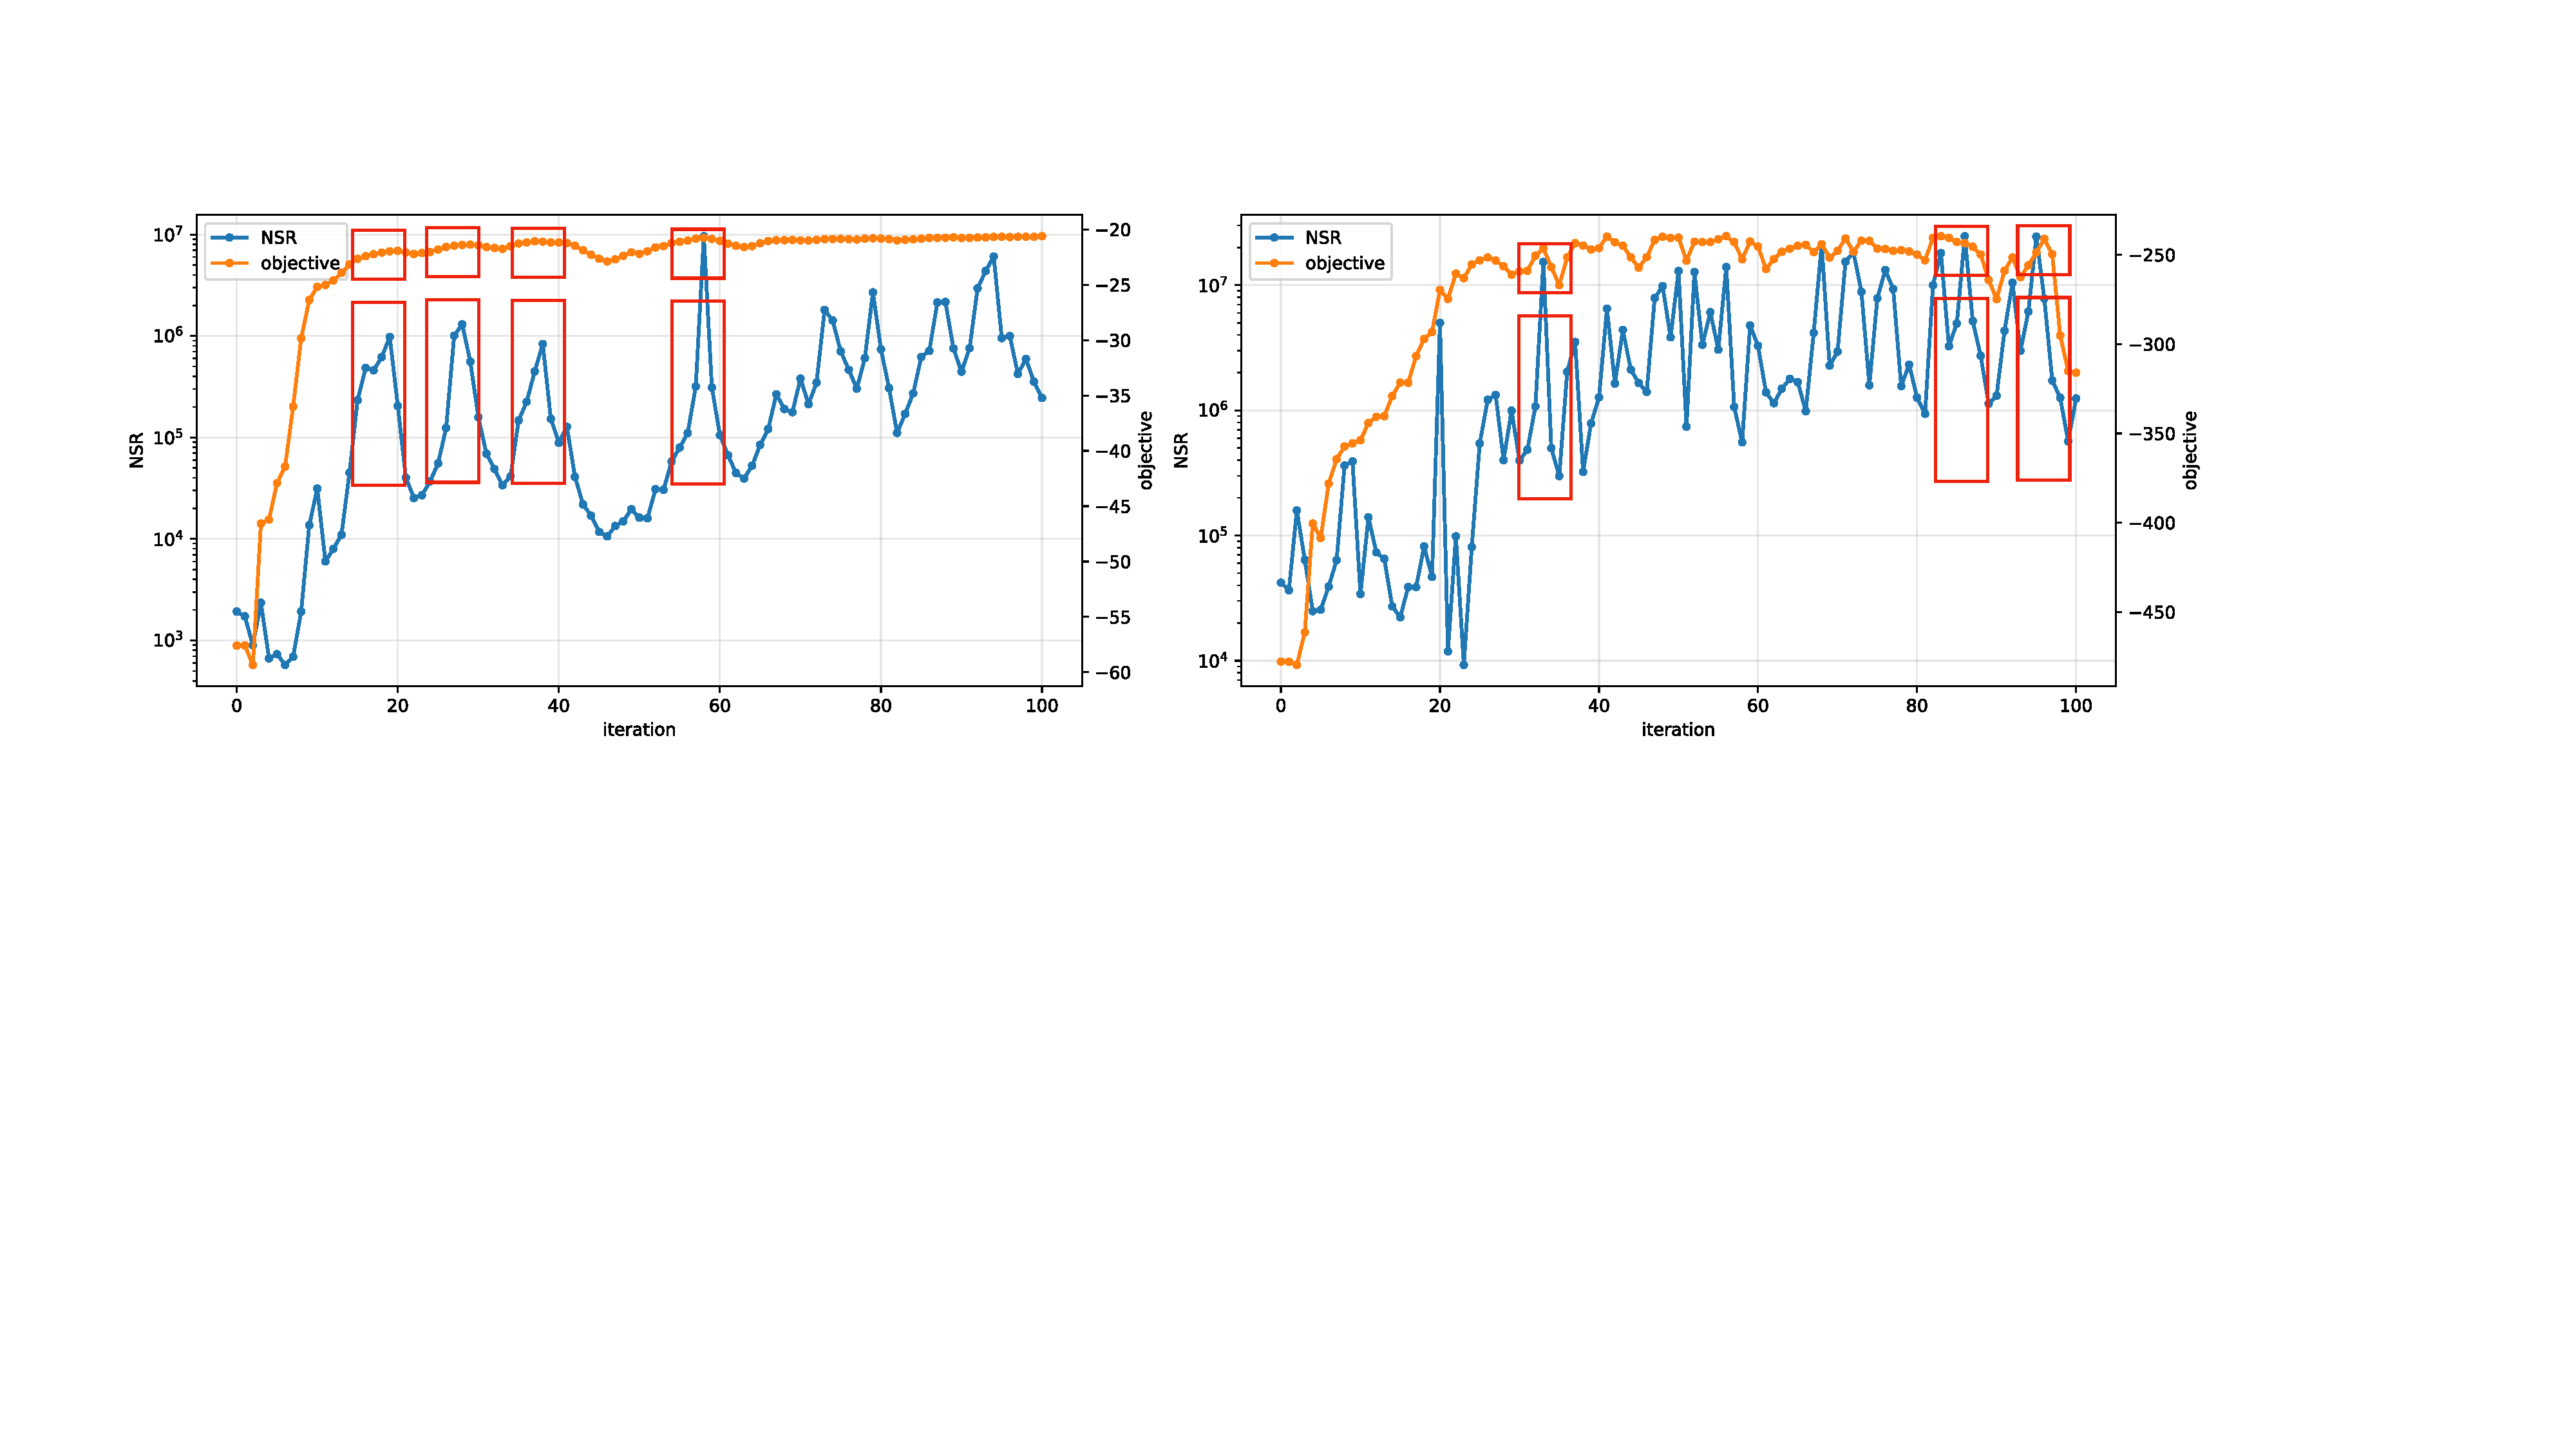
\includegraphics[width=0.9\textwidth]{figure/nonlinear_traj.pdf}
    \caption{Trajectory of NSR and objective for LQR with MLP policy (left) and Pendulum with MLP policy (right). Both the NSR and the objective are calculated through Monte Carlo evaluation. The NSR increases when approaching the optimal policy, and the red square shows the synchronized fluctuations in objective and NSR.}
    \label{fig:nonlinear-traj}
    \vspace{-2mm}
\end{figure*}


We then consider polynomial dynamics with polynomial reward, and a Gaussian policy with polynomial mean
\begin{align}\label{eq:poly-dynamics-reward}
s_{t+1}=P(s_t,a_t),\quad \pi(a\mid s)=\mathcal N \big(\Phi(s)^\top\theta,\Sigma\big),
\end{align}
where $\Phi(s)\in\mathbb R^{d\times m}$ is a matrix of polynomial features. Equivalently,
$a_t=\Phi(s_t)^\top\theta+\varepsilon_t$ with $\varepsilon_t\sim\mathcal N(0,\Sigma)$. The initial state satisfies $s_0\sim\mathcal N(0,\Sigma_0)$.

\begin{proposition}[Polynomial form of REINFORCE and exact Gaussian-moment evaluation]\label{prop:poly-isserlis}

The following statements hold for the polynomial system~\eqref{eq:poly-dynamics-reward}:

\textbf{(i) Polynomial estimator.}
For each $t\le T$, the random variables $s_t$ and $a_t$ are vector-valued polynomials in
$\xi:=(s_0,\varepsilon_0,\ldots,\varepsilon_{T-1})$. Consequently, $\widehat G_\theta$ and $\widehat G_\ell$ are polynomials in $\xi$.

\textbf{(ii) Exact moments.}
$\E[\widehat G_\theta], \E[\widehat G_\ell]$, $\E[\|\widehat G_\theta\|_{\mathrm{F}}^2]$, $\E[\|\widehat G_\ell\|_{\mathrm{F}}^2]$
are exactly computable from $\mathrm{Cov}(\xi)$ via Isserlis theorem.
\end{proposition}

Proposition~\ref{prop:poly-isserlis} shows the NSR can in principle be computed symbolically for polynomial systems. 

However, the worst-case complexity grows rapidly with the dimension, degree, and horizon. Let $P$ have degree $d_P$, $\Phi$ have degree $d_\Phi$, and $r$ have degree $d_r$. Then $\deg s_t\approx\!d_P^t d_\Phi^t$ and $\deg a_t\approx\!d_P^t d_\Phi^{t+1}$. Thus, the REINFORCE estimator involves Gaussian moments up to order $d_P^{2T} d_\Phi^{2T+1} d_r$. In the worst case, the number of monomial terms can be as large as $\binom{n + mT + d_P^{2T} d_\Phi^{2T+1} d_r}{d_P^{2T} d_\Phi^{2T+1} d_r}$, leading to exponential dependence in $T$ and a combinatorial blow-up in $n$ and $m$.

\textbf{Experiments}. We implement code to compute the objective, gradient, and variance for two polynomial systems:

\emph{Quadratic system:} $s_{t+1}=s_t+ h(-s_t^2 + a_t)$ with reward $r(s,a)=-s^2-a^2$; where $h=0.05$ is the step size. The policy is parameterized as $a_t=\theta_1 s_t + \theta_2 s_t^2 + \varepsilon_t$. 

\emph{Cubic system:} $s_{t+1}=s_t + h(-s_t^3 + a_t)$ with reward $r(s,a)=-1.25s^6 - a^2$; where $h=0.05$. The policy is parameterized as $a_t=\theta_1 s_t + \theta_2 s_t^3 + \varepsilon_t$. Note the optimal policy can be proved to be an odd function because of the symmetry of dynamics and initial state distribution.

The cubic example is motivated by an infinite-horizon continuous-time analogue where the optimal feedback is polynomial.
For $\dot s = -s^3 + a$ and the selected cost ($-r(s,a)$), the Hamilton-Jacobi-Bellman equation admits a polynomial value function $V(s)= 0.25 s^4$ and the stationary optimal policy $a^\star(s)= -0.5\,V'(s)= -0.5 s^3$.

Due to limited computational resources, we set the horizon $T=6$ for the quadratic system and $T=3$ for the cubic system. Initial state covariance is set as $\Sigma_0=0.1$.

We plot the NSR heatmap for both systems in Figure~\ref{fig:poly-variance-traj}. As in the LQG case, we examine the trajectories of three optimizers (GD, SGD, Adam) in a 3D policy-parameter space (two polynomial coefficients and one log-std). The trajectories show the same trend: the NSR increases as the policy approaches optimality. This provides evidence that the non-uniform variance / NSR phenomenon exists across different systems.

With smaller batch sizes and larger learning rates, we observe policy collapse: even near the optimum, a single noisy gradient step can drive the log-standard deviation downward, causing the NSR to blow up and the policy to collapse (Figure~\ref{fig:policy_collapse}). We further verify that this collapse is caused by statistical error by comparing against two baselines: a larger batch size and the exact gradient. The larger-batch setting still collapses, but only after a longer time, whereas the exact-gradient setting does not collapse at all (Figure~\ref{fig:policy_collapse_compare}).

\begin{figure*}
    \centering
    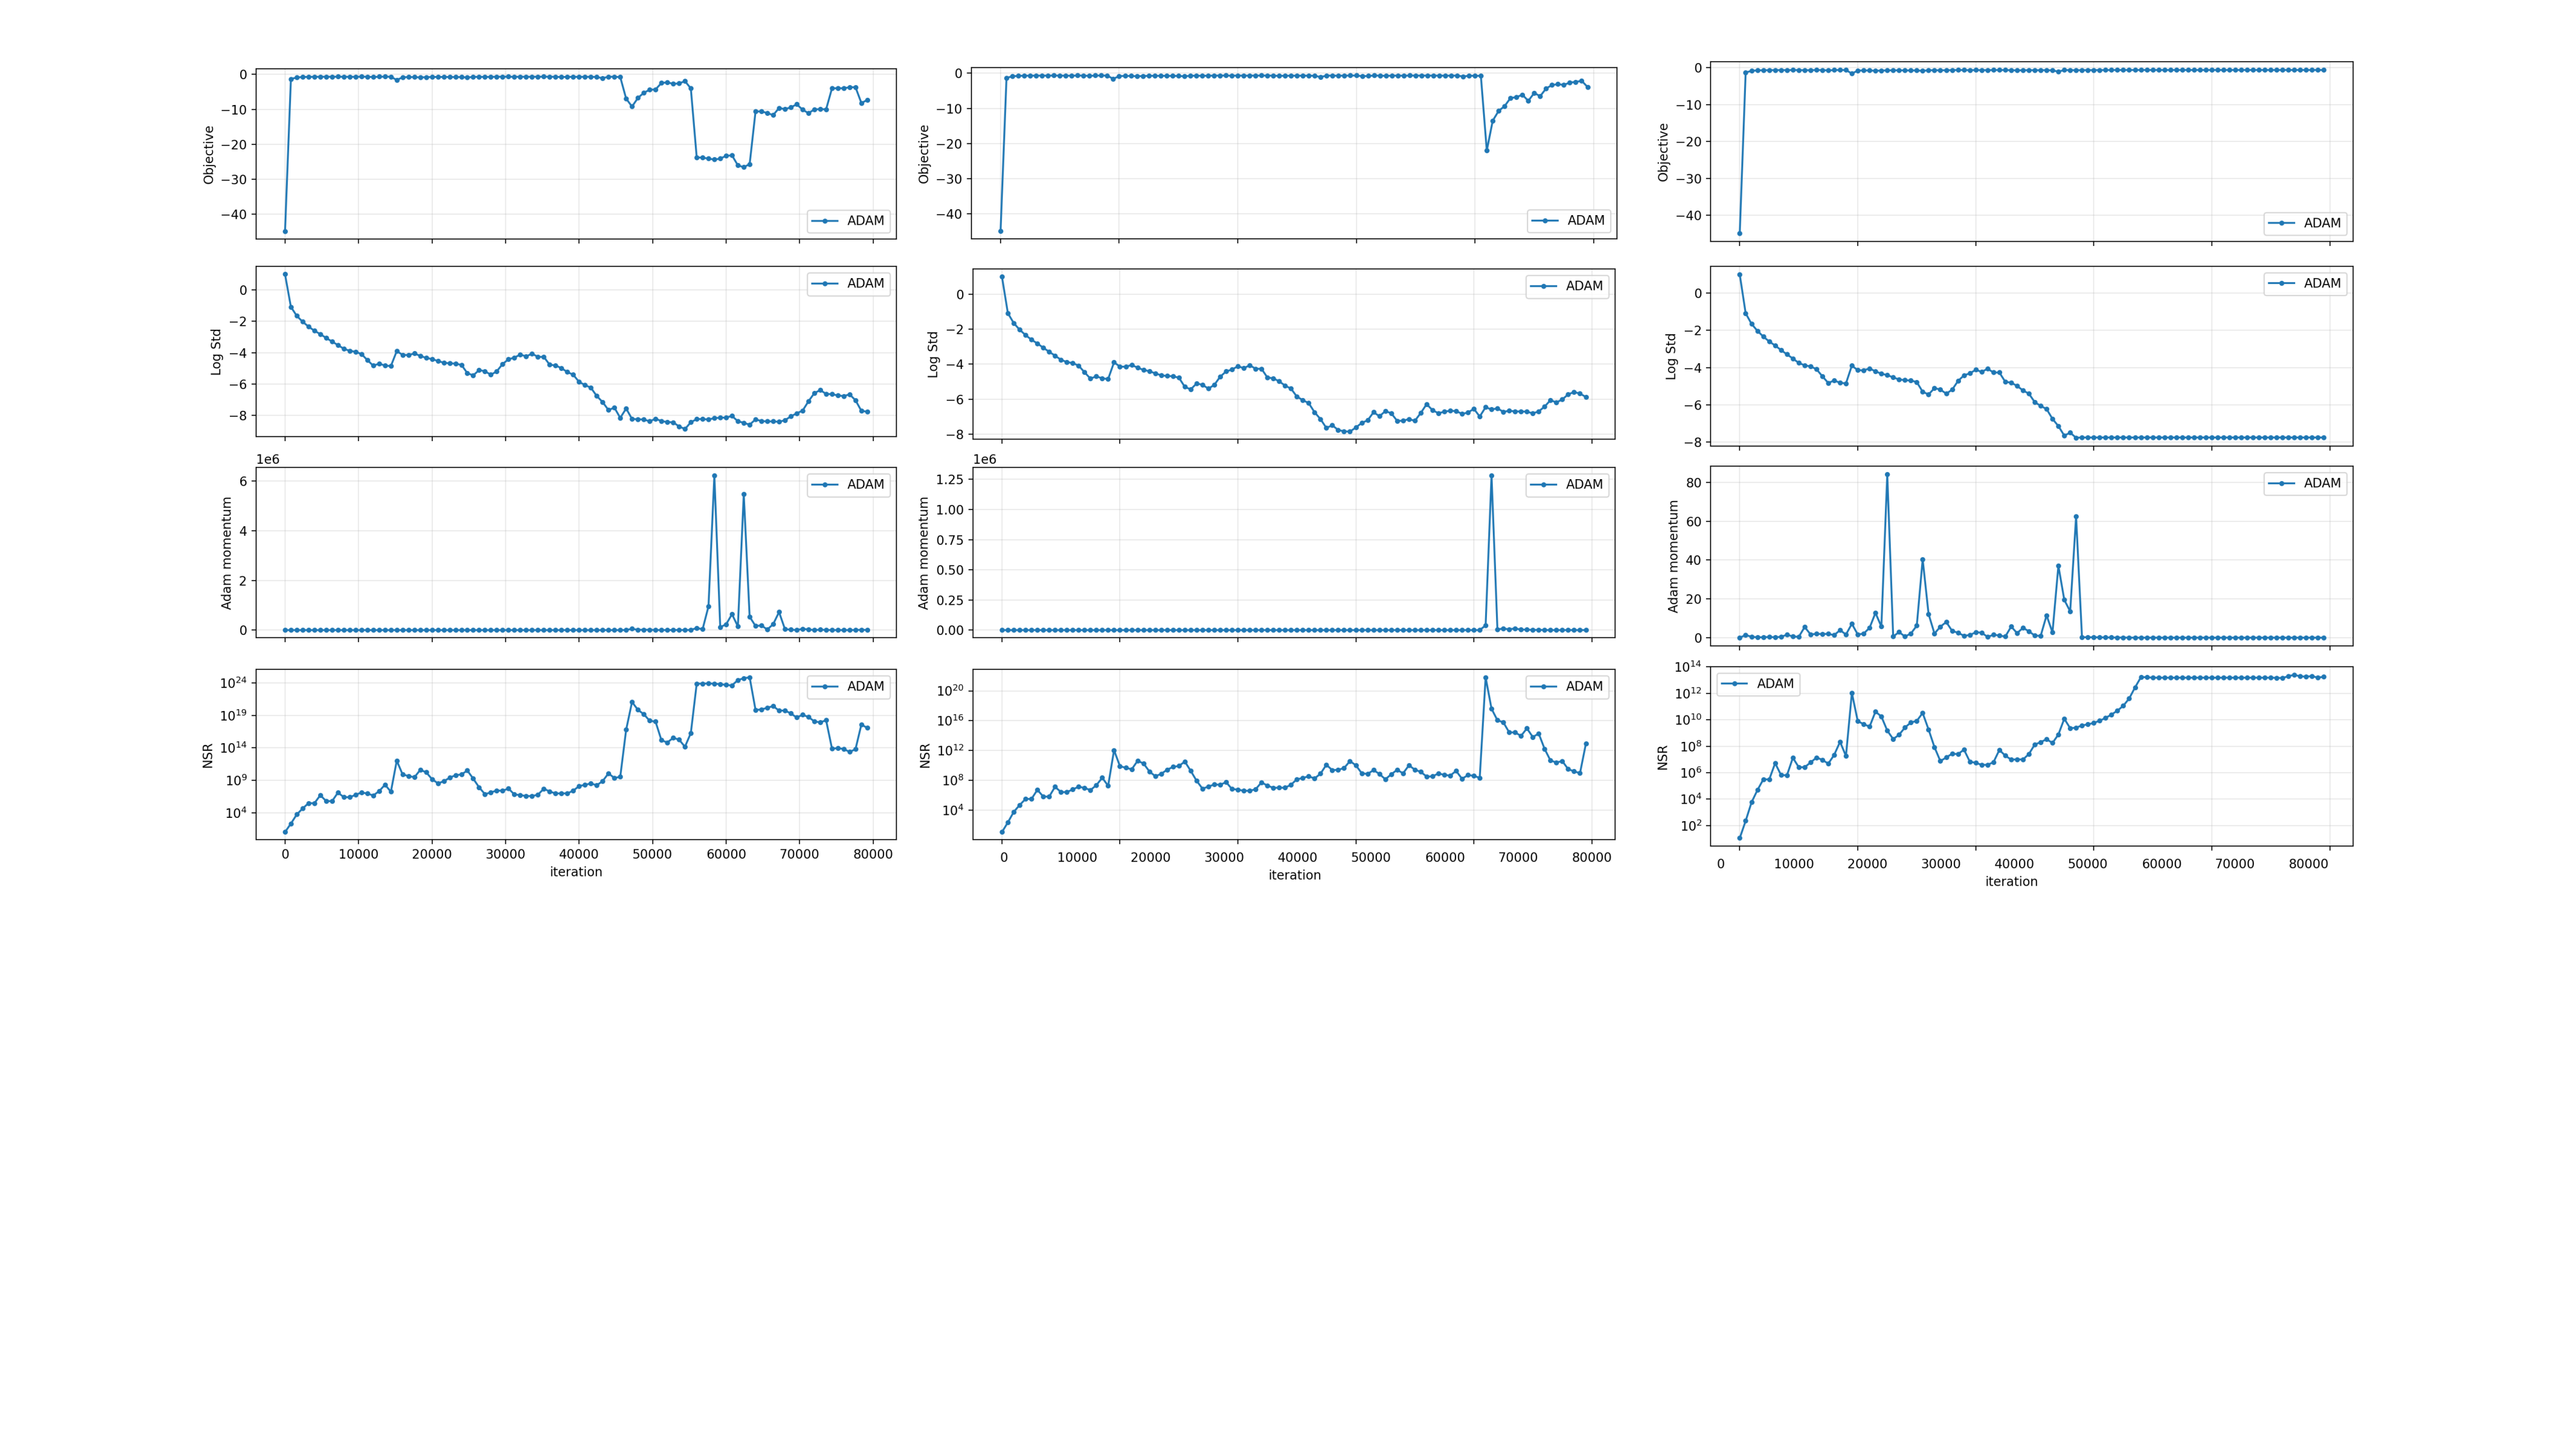
\includegraphics[width=0.88\textwidth]{figure/policy_collapse_compare.pdf}
    \vspace{-2mm}
    \caption{Detailed ablation study of policy collapse on the quadratic system. Left: original policy-collapse curves. Middle: with a larger batch size, the policy still collapses but takes longer. Right: with the exact gradient, the policy does not collapse. From top to bottom, the rows show the objective, the log-standard deviation of the policy covariance, Adam's momentum, and the NSR. These results confirm that the collapse is caused by statistical error.}
    \label{fig:policy_collapse_compare}
    \vspace{-5mm}
\end{figure*}
